\documentclass[format=final, language=chinese, degree=bachelor]{hustthesis}

\usepackage[colorinlistoftodos,prependcaption]{todonotes}

\stuno{U201315168}
\schoolcode{10487}
\title{基于Android平台的网络防火墙的设计与实现}{An Implementation of Android Firewall}
\author{易亚洲}{Yazhou Yi}
\major{信息安全}{Information Security}
\supervisor{李平}{Ping Li}
\date{2017}{6}{1}

\zhabstract{
	介绍还没有写
}

\zhkeywords{防火墙, 安卓}

\enabstract{
 The introduce is not ready
}

\enkeywords{Firewall, Android}

\graphicspath{ {images/} }

\begin{document}

\frontmatter
\maketitle
\makeabstract
\tableofcontents
\listoffigures
\listoftables
\mainmatter

\chapter{绪论}\label{chapter:1}
\section{项目背景}

\subsection{Android系统}
Android是由Google开发的一个基于Linux内核的开源操作系统,目前主要应用于手机,平板电脑,电视,车载电脑等移动设备,。Android大部分代码使用Apache 2.0协议开源,使得各大厂商都可以基于Android系统进行二次开发,打造出多种多样的Android系统,例如小米公司的MIUI,华为EmotionUI等,这些Android系统的各种深度定制版给了用户很多种选择。

Android操作系统在智能手机的市场份额自从发布以来一直保持持续上升。
在推出后两年,即2010年末,市场占有率超越塞班系统,成为全球第一大智能手机操作系统,
2016年第三季度最新数据显示,Android市场份额已经达到了86.8\%,远远超过其他操作系统的总量,并且份额将会长期保持。不像iOS操作系统,Android每年都有数以百计的合作厂商发布大量新的机型,例如Oppo,三星,华为等,用户有着大量的选择。Data: Strategy Analytics, Q3 2016, https://qz
.com/826672/android-goog-just-hit-a-record-88-market-share-of-all-smartphones/

Android操作系统本身开源的特性和在智能手机市场上的火热,让Android系统的生态系统极度丰富。同样是Android系统,不同公司定制的版本往往有着不一样的交互界面,也有着不同的自带应用。Android用户可以在应用市场选择下载数以百万计的App。但这也带来了碎片化的问题,在系统版本上,Android发布的新版本难以快速普及,大量用户仍然使用陈旧的版本,截止2016年末,接近50\%的用户仍然在使用2014年和更久以前发布的版本。这不仅给开发者带来了兼容性上的困难,也导致了巨大的安全隐患:旧版本用户系统上的安全漏洞得不到修复,新的安全机制无法生效。同时,各种定制Android的厂商的技术实力参差不齐,存在很多粗制滥造的二次开发版本,其安全性得不到任何保障。


\section{研究意义}

随着智能手机的普及,以及4G网络的快速发展,越来越多的用户开始使用手机上网冲浪。中国互联网络信息中心(CNNIC)发布了第38次《中国互联网络发展状况统计报告》。《报告》显示,截至2016年6月,中国网民规模达7.10亿,其中手机网民规模达6.56亿,占比达92.5\%。中国各类第三方市场鱼龙混杂,管理混乱,对应用上架的审核存在不规范,不严格甚至完全没有审核的现象。

根据赛门铁克(Symantec)最新互联网安全威胁报告称,在所有的安卓应用程序中有17\%是恶意软件。特别是Google Play市场无法提供服务的地区,用户不得不从未知来源下载安全应用,各种第三方市场鱼龙混杂,其中有很多恶意软件混迹其中,也有很多安全性低容易收到攻击的应用。

\begin{figure}[h!]
\centering
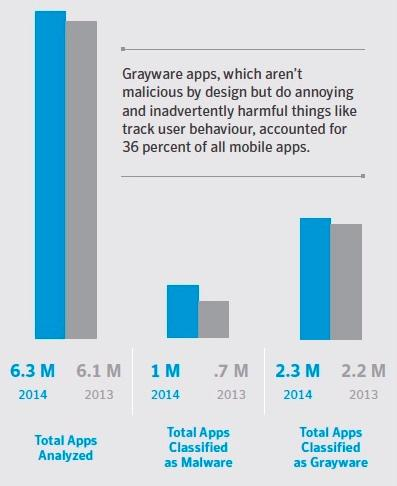
\includegraphics[width=.4\textwidth]{symantec_report}
\caption{Symantec恶意软件数量报告}\label{fig:2}
\end{figure}

腾讯移动安全实验室发布了2016年手机安全报告,报告显示2016年Android病毒包共增加2341.8万,同比增长40.20\%。2016年Android手机病毒感染用户数同比增长62.43\%,感染用户数总量达到5亿人次,达到历年新高。其中资费消耗类占比高达84.24\%,在2016年手机病毒类型中排名第一。
资费消耗类的病毒是指的在未经用户授权的情况下,通过频繁连接网络、发送短信等方式,导致用户资费损失。这部分病毒往往帮助一些广告商提高App装机量或点击率进行恶意推广,不断联网下载,消耗用户流量。

针对资源消耗类病毒,网络防火墙可以启动有效的防范和遏制的作用,将不可信应用的网络权限进行限制,对可疑应用的数据通信进行监控,是遏制这类病毒的最重要手段。此外,对于远程控制、隐私窃取等类型的软件,限制网络通信也是有效可行的重要举措。

Android系统自带的通信权限管理仅仅允许对特定应用设置是否允许链接网络,无法对Wifi网络和蜂窝数据网络区分设置,也不支持多种条件下的自定义规则,如灭屏和亮屏,特定网络,限制时段等条件,而且,不支持按协议过滤,按源目的地址过滤等基本防火墙功能。所以我们有必要开发一款Android网络防火墙来完善这些功能,满足用户对Android网络管理更高级的需求。
所以在目前Android用户数量持续增长,资费消耗病毒日渐猖獗,而Android系统网络功能不全的情况下,所以我们提出了设计并实现一个基于Android平台的网络防火墙的课题,旨在通过对Android系统网络通信的监控和管理的实现,研究Android网络安全,设计一个可用的Android网络防火墙,改善Android系统的安全性。

\section{预期目标}

本论文的目标是通过设计和实现一个Android网络防火墙,通过对Android系统网络通信的监控和管理,提高Android系统的安全性,有效防范资费消耗类恶意软件。目前存在多种Android防火墙的实现方案,但我们希望避提供一个普通Android用户下载安装后即可用的解决方案,而不是要求提取系统Root权限,甚至定制操作系统内核等难以实行的方案。本文采取的设计方案不是类似传统防火墙由管理员设定一组规则然后一直照此执行直到修改规则,而是采用交互式规则,在应用尝试进行一些网络请求时,通知用户做出决策:允许或者拒绝,并且即时的更新规则。同时需要监控连接的流量消耗,提供地址的相关信息,为用户做出决策提供帮助。


最后,将针对防火墙的性能,对处理每个包时引入的能耗,包丢失和延迟进行基准测试。通过分析证明,使用这样的防火墙是可行的,并且不影响Android设备的日常功能。

\section{需求分析}

\todo[inline]{需求分析还需要扩充,参考discowall,加入项目目标和用户分析开发环境和时间安排内容,扩充至两页}

在对市场上多款防火墙类应用软件进行分析和比较之后,将用户需求列为以下几点:
\begin{itemize}
	\item 过滤Android系统所有流量\label{item:1}
	\item 图形界面,操作简便,通俗易懂
	\item 支持WiFi和数据流量应用不同规则
	\item 支持亮灭屏状态应用不同规则
	\item 支持分时段应用不同规则p
\end{itemize}

对于上述需求,进行明确和细化,方便开发和测试验收:
\subsection{功能性要求}
\subsubsection{兼容和适配}
	
	兼容到Android4.0及以上
\subsubsection{防火墙}
\begin{enumerate}
	\item 交互式规则:如果新建立的连接没有已知的规则进行决策,会通知用户即时作出决策。在用户可以在弹出的通知栏里选择允许或者拒绝,然后就会记住该规则,在以后有相同的连接时采用该规则;如果用户选择了拒绝,该连接将会被切断。
	\item 审计式规则:用户可以查看近期所有的连接记录,可以选择对特定连接快捷建立规则
	\item 规则的适用范围:
		\begin{itemize}
			\item 面向应用:用户可以设定规则只对特定应用生效
			\item 面向出口:用户可以设定规则只对特定网络环境生效,如Wifi/2G/3G/LTE/漫游
			\item 面向特定状态:用户可以设定规则只对特定手机状态生效
		\end{itemize}
	\item 防火墙默认策略:当用户没有为特定应用设定规则时,采用默认策略
	\item 实时网速监控:用户可以在通知栏查看实时的网速
	\item 新应用提示:在用户安装新的应用程序后,会提示用户为其创建规则
\end{enumerate}

\subsubsection{性能}

网络防火墙为了提供额外的安全保障,必须尽可能的持续运行。所以网络防火墙必须对Android移动设备的的性能和电量的消耗保持在最小。所以必须采取措施将防火墙规则匹配的耗时和对包处理的耗时降到最低,例如TCP连接可以只对SYN和FIN包进行处理便可实现监控TCP连接的生命周期,此外我们还需对其他协议及在所有可能的环节降低性能损失,并通过性能测试和报告证明防火墙对设备所造成的性能损失在可以容忍的较小范围之内。

\subsection{非功能性要求}

为了提高体验和方便实际使用,还需实现一些非核心功能的特性:
\begin{enumerate}
	\item 日志查看:记录应用程序的网络访问尝试
	\item 支持系统应用:支持对系统应用设置规则
	\item 支持IPv6:提供对IPv6及ICMPv6的支持
	\item 端口转发:支持增加/删除/编辑端口转发规则
	\item 配置导入导出:支持将规则和配置导出到文件或者从文件中导入
	\item 持久有效:防火墙必须持续有效的工作:\begin{itemize}
		\item 进程必须尽可能避免被系统停止或杀死
		\item 防火墙必须在断开时尝试重新启动
		\item 防火墙必须在开机自动启动
	\end{itemize}
\end{enumerate}


\section{进度安排}

项目的工作主要安排在2017年2月13日至2017年5月22日。相关重要时间点如下:
\begin{enumerate}
	\item 开题,第四周前(2017年3月10日前)
	\item 中期检查,第九周前(2017年4月10日前)
	\item 完成论文编写,第15周前(2017年5月22日前)
	\item 答辩和验收,第18周前(2017年6月16日前)
\end{enumerate}

具体时间及任务安排如下:

\begin{table}[h!]
\centering
\caption{研究进度安排表}
	\begin{tabular}{|c|l|l|}\hline
	周次 	& 日期 & 任务安排\\\hline
	1		& 2.13~2.19 & 收集相关文献,对Android安全和防火墙技术的最新研究进行了解,编写文献综述\\\hline
	2		& 2.20~2.26 & 体验和研究现有的防火墙应用,进行市场调查\\\hline
	3		& 2.27~3.5  & 完成需求分析,确定方案可行性,了解项目要求的技术知识\\\hline
	4		& 3.6 ~3.10 & 完成开题报告\\\hline
	5		& 3.11~3.19 & 完成好相关准备工作,进行总体模块划分,确定各模块的总体设计\\\hline
	6,7		& 3.20~4.2  & 编码实现,完成核心功能\\\hline
	8,9 	& 4.3 ~4.16 & 编码实现图形界面\\\hline
	10		& 4.17~4.23 & 进行基本功能的测试\\\hline
	11,12	& 4.24~5.7  & 增加更多功能,完善兼容性,性能优化和改善易用性\\\hline
	13 		& 5.8 ~5.14 & 进行完整的功能测试,兼容性测试和性能测试\\\hline
	14 		& 5.15~5.22 & 对开发工作进行整理,编写论文报告\\\hline
	\end{tabular}	
\end{table}


\section{内容概括}

\todo[inline]{增加对分章节概括的的一节}

\chapter{设计原理}\label{chapter:3}

\section{Android系统架构}

Android操作系统的核心是Linux内核的一个分支,但也有很多的修改和扩充。其中主要包括:去除了X Windows System,不支持GNU库。另外主要增加了两个部分,Binder IPC和Wakelock管理。
\todo{Android架构仍有扩充空间}

Android系统的架构如图所示,分为四层,自上而下分别是应用程序(Applications),应用程序框架(Application Frameworks),系统运行库与Android运行环境(Libraries \& Android Runtime),Linux内核(Linux Kernel)。
\begin{itemize}
\item 应用程序层由各种应用软件组成,如短信,浏览器,地图等,这些应用可以是系统自带,也可以是从应用市场下载。
\item 应用程序框架层提供了应用程序运行需要的各种API和系统服务,主要由Java编写。开发者开发Android应用需要对这一层由较多的了解。它提供了用于实现图形界面的视图,活动管理器,窗口管理器,内容提供者,资源管理器,通知管理器,包管理器,等。
\item Android运行库是为Android系统中各种组建运行而提供的C/C++库的合集,用以实现底层的图形绘制,媒体播放录制,Web页面渲染,3G图形,SQLite数据库等功能。而Android运行时则是Android虚拟机的实现,Android 5.0以前是Dalvik虚拟机,5.0以后是ART虚拟机,用以执行应用软件中的字节码。
\item Linux内核为Android提供硬件驱动,内存管理,进程眼里,网络协议栈和安全体系等实现。同时,Android加入了针对移动设备优化的电源管理和Binder机IPC机制。
\end{itemize}
https://hit-alibaba.github.io/interview/Android/basic/Android-Arch.html

\section{实现策略}
实现对Android流量的过滤,有多种实现方式,Android内核是linux内核的一种分支,也提供netfilter和iptable,可以参考Linux内核防火墙的实现方式实现Android防火墙。

\subsection{Netfilter防火墙}

https://www.ibm.com/developerworks/cn/linux/network/l-netip/

Netfilter是Linux 2.4.x之后版本提供的包过滤的框架,它在TCP/IP协议栈中提供了相应的Hook,允许我们对网络数据包进行过滤,丢弃,修改等操作。通过netfilter中的一些函数即可实现防火墙应用。而iptables是linux提供的一个基于netfilter工具,使用户可以对整个操作系统收发的数据包就行拦截修改拒绝等操作。
以IPv4为例,netfilter在IPv4协议栈中定义了五个hook,在这五个点使用nf\_hook\_ops结构注册hook,过滤经过该点的所有包,nf\_hook\_ops定义如下:

\begin{lstlisting}[language=c]
struct nf_hook_ops
{
    struct list_head list;
    nf_hookfn *hook;
    int pf;
    int hooknum;
    int priority;
};
\end{lstlisting}

nf\_hook\_ops中的nf\_hookfn就是hook函数,实现一个nf\_hookfn函数,在该函数中实现对包的读取解析并过滤,返回NF\_ACCEP,NF\_DROP等返回值,即可实现对数据包的操作。

\subsection{VPN防火墙}

Android系统本身提供了制作VPN应用的API,允许第三方应用向系统提供VPN,系统负责将网络流量转发到VPN应用,VPN应用可以建立隧道实现VPN服务。而在这个过程中,VPN应用可以对网络流量进行分析和过滤,实现防火墙的功能。

\subsection{方案对比}
netfilter/iptable需要调用netfilter api或执行iptable,这都必须拥有root权限才有可能实现。Root本身就是利用漏洞才得以实现的,并且root之后的手机毫无安全性可言,与我们做防火墙提高安全性的初衷相悖。

VPN方案由于使用了Android官方提供的公开API,可以不需要Root权限运行,只需要用户在第一次启动VPN时授予许可,也没有给系统带来额外的安全风险。其缺陷在于VPN服务只允许启动一个,将会导致用户使用防火墙后无法使用其他VPN。

以加强Android安全作为出发点,通过对两种方案的对比,我们最后决定采用VPN方案实现Android防火墙。

\section{开发环境}

Google为开发Android应用程序提供了一系列的开发工具。
\todo{列举开发工具}

\section{VpnService API}

VpnService是用来继承并实现自己的VPN应用的基础类。它创建了虚拟网络接口,配置地址和路由规则,返回一个文件描述符给应用。对文件描述符每一次读,就会读取一个通过这个接口向外发出的数据包;对文件描述符的每一次写,就会插入一个入数据包,对接口而言,就相当于这个接口接收到了这个数据包/这个虚拟网络接口运行于IP协议层,所以数据包的 开头都是IP数据头。通过这个API,应用可以实现在隧道中与远程服务器的数据包处理和交换,构造一个VPN应用。

允许应用拦截数据包带来了巨大的安全隐患。一个VPN应用可以轻而易举的切断网络,此外多个VPN应用也可能互相冲突。系统采取了多种措施来解决这个问题。主要是:
\begin{enumerate}
 	\item 第一次创建VPN链接的时候,必须需要用户的授权;\label{item:1}
	\item 同时只能有一个VPN运行。如果创建一个新的连接,现有的连接都会被切断;
	\item 在VPN运行的全程,都会有一个系统级的通知显示在通知栏告知用户;
	\item 系统会提供一个系统级的对话框,告知用户当前VPN连接的信息并允许用户断开VPN连接;
	\item 当文件描述符关闭的时候或VPN应用崩溃和被系统杀死的时候,网络状态会被自动还原。
\end{enumerate}

VpnService中有两个重要方法:

\begin{lstlisting}[language=Java]
prepare(Context);
establist();
\end{lstlisting}

前者处理用户的行为和停止其他应用的VPN连接,后者通过VpnService.Builder提供的参数创建VPN连接。应用必须调用 prepare(Context)确保取得对当前类其他方法的授权。这个授权随时可能被收回。创建一个VPN连接的步骤如下:
 \begin{enumerate}
     \item 当用户按下连接的按钮时,调用prepare(Context),并且在这个方法返回的intent非空时启动这个intent;这个方法为了取得用户的授权,这个方法返回null时说明用户此前已经授权过;
     \item 当用户授权之后,启动VpnService服务;
     \item 创建一个到远程服务的隧道,并且交换vpn连接的参数并配置好;
     \item 将这些参数应用到 VpnService.Builder , 并通过调用establish()创建VPN接口;
     \item 在隧道和返回的文件描述符之间处理和交换信息;
     \item 当onRevoke()收回权限时,关闭文件描述符和隧道。
\end{enumerate}

 应用在继承VpnService实现VPN必须声明相应的权限和intent过滤器,范例如下:
\begin{lstlisting}[language=xml]
  <service android:name=".ExampleVpnService"
          android:permission="android.permission.BIND_VPN_SERVICE">
      <intent-filter>
          <action android:name="android.net.VpnService"/>
      </intent-filter>
  </service>
\end{lstlisting}


\section{处理通信流量}

在我们的应用中,不需要创建一个到远程服务的隧道,但需要处理文件描述符中的数据。我们需要从文件描述符读取发送出来的流量,将其分析过滤,然后将其标记,然后写回文件描述符。这个过程使用C语言调用Android NDK API完成,然后通过JNI在Java代码中调用。首先,需要对文件描述符进行操作。

\subsection{文件描述符的操作}

https://segmentfault.com/a/1190000003063859

文件描述符是一个用于表述指向文件的引用的抽象化概念。我们需要对Vpn创建后返回的文件描述符进行操作,从中读取数据包进行处理。我们采用epoll机制进行文件描述符的监听,以下为需要使用的函数:

\begin{lstlisting}[language=c]
int epoll_create(int size);//创建一个epoll文件,size用来告诉内核这个监听的数目一共有多大
int epoll_ctl(int epfd, int op, int fd, struct epoll_event *event);
int epoll_wait(int epfd, struct epoll_event * events, int max_events, int timeout);
\end{lstlisting}

\begin{enumerate}
\item \lstinline {int epoll\_create(int size); }

创建一个epoll的句柄,size用来告诉内核这个监听的数目一共有多大,参数size并不是限制了epoll所能监听的描述符最大个数,只是对内核初始分配内部数据结构的一个建议。当创建好epoll句柄后,它就会占用一个fd值,在linux下如果查看/proc/进程id/fd/,是能够看到这个fd的,所以在使用完epoll后,必须调用close()关闭,否则可能导致fd被耗尽。

\item
\lstinline {int epoll\_ctl(int epfd, int op, int fd, struct epoll\_event *event);}

函数是对指定描述符fd执行op操作。
	\begin{itemize}
		\item epfd:是epoll\_create()的返回值。\label{item:2}
		\item \verb|op:表示op操作,用三个宏来表示:添加EPOLL_CTL_ADD,删除EPOLL_CTL_DEL,修改EPOLL_CTL_MOD。分别添加、删除和修改对fd的监听事件。|
		\item fd:是需要监听的fd(文件描述符)
		\item epoll\_event:是告诉内核需要监听什么事,struct epoll\_event结构如下:
		\begin{lstlisting}[language=c]
struct epoll_event {
  __uint32_t events;  /* Epoll events */
  epoll_data_t data;  /* User data variable */
};
		\end{lstlisting}
	events可以是以下几个宏的集合:
		\begin{itemize}
			\item EPOLLIN :表示对应的文件描述符可以读(包括对端SOCKET正常关闭);\label{item:3}
			\item EPOLLOUT:表示对应的文件描述符可以写;
			\item EPOLLPRI:表示对应的文件描述符有紧急的数据可读(这里应该表示有带外数据到来);
			\item EPOLLERR:表示对应的文件描述符发生错误;
			\item EPOLLHUP:表示对应的文件描述符被挂断;
			\item EPOLLET: 将EPOLL设为边缘触发(Edge Triggered)模式,这是相对于水平触发(Level Triggered)来说的。
			\item EPOLLONESHOT:只监听一次事件,当监听完这次事件之后,如果还需要继续监听这个socket的话,需要再次把这个socket加入到EPOLL队列里
		\end{itemize}
	\end{itemize}
\item \lstinline {int epoll\_wait(int epfd, struct epoll\_event *events, int max_events, int timeout);}
等待epfd上的io事件,最多返回max\_events个事件。

参数events用来从内核得到事件的集合,maxevents告之内核这个events有多大,这个maxevents的值不能大于创建\verb|epoll_create()|时的size,参数timeout是超时时间(毫秒,0会立即返回,-1将不确定,也有说法说是永久阻塞)。该函数返回需要处理的事件数目,如返回0表示已超时。

调用\verb|epoll_wait|时,线程会堵塞直至得到事件或者超时。其返回值i表示就绪的文件描述符的数目,当其大于0时,我们需要遍历events数组,数组里包含i个已经就绪的文件描述符。从就绪的文件描述符读取数据后进行解析和处理。
\end{enumerate}

\subsection{IP数据包处理}

%% http://www.ciscopress.com/articles/article.asp?p=348253&seqNum=4

从文件描述符读取的数据是IP数据包,IP数据包中包含了将数据在因特网上路由和传输的必要的信息,这部分信息存在于IP首部中
,对我们的应用格外重要的包括IP协议版本,源IP,目的IP等信息,我们需要实现对IP头的解析,以便于应用过滤规则。IP协议分为IPv4和IPv6,需要分别解析。

IPv4报文的首部包含13个必须字段,1个可选字段。所有字段均为大端的二进制顺序。IPv4首部结构如表\autoref{tab:1}所示:

\begin{table}[h!]
\centering
\caption{IPv4首部结构}\label{tab:1}
\begin{tabular}{|c|c|c|c|c|c|c|}
	\hline
	位偏移 & 0-3 & 4-7 & 8-13 & 14-15 & 16-18 & 19-31\\
	\hline
	0 & 版本 & 首部长度 & DSCP & 显式拥塞通告 & \multicolumn{2}{c|}{全长}\\
	\hline
	32 & \multicolumn{4}{c|}{标志符} & 标志 & 分片偏移 \\
	\hline
	64 & \multicolumn{2}{c|}{存活时间}& \multicolumn{2}{c|}{协议}& \multicolumn{2}{c|}{首部检验和} \\
	\hline
	96 & \multicolumn{6}{c|}{源IP地址} \\
	\hline
	128 & \multicolumn{6}{c|}{目的IP地址} \\
	\hline
	160 & \multicolumn{6}{c|}{选项(如首部长度>5)} \\
	\hline
	160 or 192+ & \multicolumn{6}{c|}{数据}\\
	\hline
\end{tabular}
\end{table}


其中值得我们关注的是:
\begin{table}[h!]
\begin{tabular}{l l}
	版本 & IP报文首部前4位是版本,我们需要对IPv4和IPv6采用不同的解析方式;\\
	首部长度(IHL) & 第二个字段是4位首部长度,说明首部有多少32位字长。\\
	协议 & 这个字段定义了该报文数据区使用的协议。IANA维护着一份协议列表(最初由RFC 790定义)。\\
	源地址 & 一个IPv4地址由四个字节共32位构成,此字段的值是将每个字节转为二进制并拼在一起所得到的32位值。\\
	目的地址 & 与源地址格式相同,但指出报文的接收端。
\end{tabular}
\end{table}


在netinet/ip.h头文件中定义了名为iphdr的结构体:
\begin{lstlisting}[language=c]
        struct iphdr {
        #if defined(__LITTLE_ENDIAN_BITFIELD)
            uint8_t  ihl    :4,
                 version:4;
        #elif defined (__BIG_ENDIAN_BITFIELD)
            uint8_t  version:4,
                 ihl    :4;
        #else
        #error	"Please fix <asm/byteorder.h>"
        #endif
            uint8_t	  tos;
            uint16_t  tot_len;
            uint16_t  id;
            uint16_t  frag_off;
            uint8_t   ttl;
            uint8_t   protocol;
            uint16_t  check;
            int32_t   saddr;
            int32_t   daddr;
        };
\end{lstlisting}

首先从pkt报文段中读取协议字段,源地址和目的地址:

\begin{lstlisting}[language=c]

        struct iphdr *ip4hdr = (struct iphdr *) pkt;

        protocol = ip4hdr->protocol;
        saddr = &ip4hdr->saddr;
        daddr = &ip4hdr->daddr;

\end{lstlisting}

还需要读取有效载荷的偏移位置payload:

\begin{lstlisting}[language=c]
         uint8_t ipoptlen = (uint8_t) ((ip4hdr->ihl - 5) * 4);
         payload = (uint8_t *) (pkt + sizeof(struct iphdr) + ipoptlen);
\end{lstlisting}

对于IPv6协议,我们需要有不同的处理方法,由于IPv6除了固定的首部(Fixed Header)存在多个扩展首部(Extension Header),所以获得载荷偏移位置较为复杂。下面为IPv6的Fiexed Header结构:


\begin{table}[h!]
\centering
\caption{IPv6固定首部结构}\label{tab:1}
\begin{tabular}{|c|c|c|c|c|c|c|}
	\hline
	位偏移 & 0-3 & 4-7 & 8-11 & 12-15 & 16-23 & 24-31\\
	\hline
	0 & 版本 & \multicolumn{2}{c|}{流量类} & \multicolumn{3}{c|}{流标签}\\
	\hline
	32 & \multicolumn{4}{c|}{负载长度} & 下一个首部的类型 & Hop限制 \\
	\hline
	64 & \multicolumn{6}{c|}{源IP地址} \\
	\hline
	192 & \multicolumn{6}{c|}{目的IP地址} \\
	\hline
\end{tabular}
\end{table}




IPv6的固定首部后,可能存在多个包含下层协议信息的扩展首部;可选的扩展首部后面才是包含上层协议信息的载荷。最后一个首部的Next Header中的值表示接下来的载荷是何种上层协议的信息,其他首部的Next Header表示下一个首部的类型。根据IPv6的相关标准,目前已经定义以下值的可选首部:



https://technet.microsoft.com/en-us/library/cc958821.aspx


\begin{lstlisting}[language=c]
        uint16_t off = 0;
        protocol = ip6hdr->ip6_nxt;
        if (!is_upper_layer(protocol)) {
            log_android(ANDROID_LOG_WARN, "IP6 extension %d", protocol);
            off = sizeof(struct ip6_hdr);
            struct ip6_ext *ext = (struct ip6_ext *) (pkt + off);
            while (is_lower_layer(ext->ip6e_nxt) && !is_upper_layer(protocol)) {
                protocol = ext->ip6e_nxt;
                log_android(ANDROID_LOG_WARN, "IP6 extension %d", protocol);

                off += (8 + ext->ip6e_len);
                ext = (struct ip6_ext *) (pkt + off);
            }
            if (!is_upper_layer(protocol)) {
                off = 0;
                protocol = ip6hdr->ip6_nxt;
                log_android(ANDROID_LOG_WARN, "IP6 final extension %d", protocol);
            }
        }
\end{lstlisting}

在完成IP层的IP首部的解析后,我们已经获知了数据包的源IP,目的IP,载荷偏移地址和传输层协议。根据协议的不同,我们还需进行进一步的解析。我们准备支持的传输层协议包括TCP,UDP,ICMP和ICMPv6协议。这些协议的值定义在linux/in.h文件中。下面我们需要对不同协议进行分别处理。

\subsection{TCP协议报文解析}

TCP(Transmission Control Protocol )提供了点对点,面向连接的可靠传输服务。TCP负责建立TCP连接,在传输过程中,TCP有序发送数据报并进行确认,对丢失的数据报进行重发恢复。我们对TCP层的数据进行解析的主要目的包括两个:
    获知TCP数据报的来源端口和目的端口
    确定TCP连接握手建立和断开的时间,用以统计网络连接时长和发送的包的大小,为用户提供流量统计等功能

TCP首部的结构如\autoref{tab:4}:

\begin{table}[h!]
\centering
\caption{TCP报文首部结构}\label{tab:4}
\begin{tabular}{|c|c|c|c|c|}
	\hline
	位偏移 & 0-3 & 4-7 & 8-15 & 16-31\\\hline
	0 & \multicolumn{3}{c|}{来源端口} & 目的连接端口 \\\hline
	32 & \multicolumn{4}{c|}{序列号码}  \\\hline
	64 & \multicolumn{4}{c|}{确认号码}  \\\hline
	96 & 报头长度 & 保留 & 标志符 & 窗口大小 \\	\hline
	128 & \multicolumn{3}{c|}{校验和} & 紧急指针 \\\hline
	160 & \multicolumn{4}{c|}{选项字段} \\\hline
	160 or 192+ & \multicolumn{4}{c|}{数据}\\\hline
\end{tabular}
\end{table}

TCP协议使用端口号进行区分发送方和接收方的应用层,我们需要实现对来源连接端口和目的连接端口进行解析读取。

如下代码可实现对端口的解析:

\begin{lstlisting}[language=c]
    char source[INET6_ADDRSTRLEN + 1];
    char dest[INET6_ADDRSTRLEN + 1];
    if (s->tcp.version == 4) {
        inet_ntop(AF_INET, &s->tcp.saddr.ip4, source, sizeof(source));
        inet_ntop(AF_INET, &s->tcp.daddr.ip4, dest, sizeof(dest));
    } else {
        inet_ntop(AF_INET6, &s->tcp.saddr.ip6, source, sizeof(source));
        inet_ntop(AF_INET6, &s->tcp.daddr.ip6, dest, sizeof(dest));
    }
\end{lstlisting}

对于TCP连接的建立和结束时间的监控过程较为复杂,需要对TCP连接的详细过程进行了解。

\subsubsection TCP状态图

TCP协议工作的过程包括三个部分:创建连接,数据传输和连接终止。这个过程中TCP连接的状态复杂,我们需要对其中的状态变化进行分析才能获知TCP连接传输的时间和数据信息。

创建连接:

LISTEN
 表示正在等待任一远程的TCP的连接
SYN-SENT
 表示已经发送SYN请求之后,正在等待对应连接的SYN请求
SYN-RECEIVED
 表示正在等待确认连接的请求,并且此时已经收到了SYN和发送了连接请求
ESTANLISHED
 表示双方据已经建立了连接,已经可以开始传输数据了
FIN-WAIT-1
 表示等待远程TCP防的连接终止请求,或先前发送的连接终止请求的确认应答
FIN-WAIT-2
 表示等待远程TCP防的连接终止请求
CLOSE-WAIT
 表示等待本地用户的连接终止请求
CLOSING
 表示等待远程TCP的连接终止请求的确认应答
LAST-ACK
 表示等待先前发送给远程TCP的终止请求的确认应答
TIME-WAIT
 表示等待过去足够的时间,确保远程TCP接收到了它发送的连接终止请求。MSL(maximum segment lifetime)用来表示TCP连接能在TIME-WAIT状态等待的最大时间,这个值的最大值为4分钟
CLOSED
  表示目前没有任何连接状态


\subsection UDP协议的处理


\subsection{伪代码}

\begin{lstlisting}
handle_events(args){

    // Terminate existing sessions not allowed anymore
    check_allowed(args)

    epoll_create

    while (!stopping) {
        分别数未关闭ICMP,UDP,TCP的数目
        if(上次检查的时间在100ms以前){

            while (s!= NULL){
                int del = 0;



            }

        }


    }


}
\end{lstlisting}

\chapter{概要设计}

\section{总体功能设计}
\todo[inline]{增加模块图,完善列举所有功能}
\todo[inline]{对所有功能进行描述,画大量的逻辑图,扩充至10页}

\subsetion{网络防护}

\subsubsection{功能设计}

用户期望一个Android防火墙应用提供友好的交互界面和正常的拦截效果。设计中应实现:
\begin{itemize}
    \item 拦截管理界面:对某个应用设置是否拦截流量
    \item 全局控制开关:切换全局防火墙状态
    \item 查看历史通信日志:查看单个应用的通信日志,包括尝试访问的地址,端口,协议类型,
    \item 设置亮屏等特殊请客的规则
    \item 支持IPv6
    \item 支持家庭网络,按流量计费网络等单独规则
    \item 配置导出导入
\end{itemize}

\subsubsection{模块设计}

根据实现防火墙的原理和功能需求,设计了成如\autoref{fig:5}的应用架构。

\begin{figure}[!h]
\centering
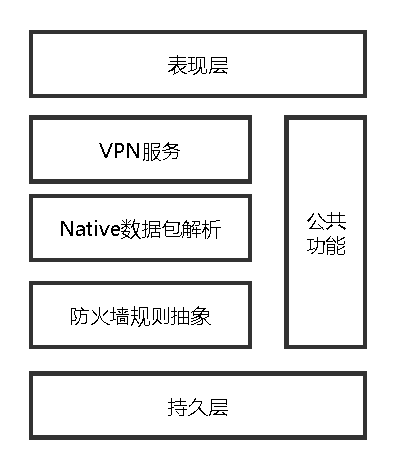
\includegraphics[width=.6\textwidth]{modules.pdf}
\caption{应用模块层次}\label{fig:5}
\end{figure}

\begin{itemize}
	\item 表现层\\ 表现层采用Activity作为主要实现,为用户提供友好的图形界面,是用户操作和管理防火墙的门户,是所有功能的入口,同时也承担着,在VPN服务层返回相应的信息(比如要求用户对是否允许某个应用的连接进行选择)时,对用户进行提醒;
	\item VPN服务模块\\该模块是继承并实现Android提供的VpnService的关键组件,用以实现VPN的功能,将VPN过滤的流量传递到下一层进行解析,并根据解析和匹配的结果,向系统回应是否作相应的处理;
	\item Native数据包解析模块\\该层主要完成将网络数据包进行解析,从中提取协议、地址、会话时间等关键信息,并用防火墙规则进行匹配,判断数据包是否放行;
	\item 防火墙规则抽象模块\\该模块负责管理持久层的防火墙规则数据,将持久层信息抽象成相应的Java对象,供Native数据包解析模块使用;同时,由于在大量数据包中,规则的读取极其频繁,防火墙规则抽象模块也负责实现对规则的缓存,提高性能;
	\item 持久层\\主要负责为上层模块提供持久化储存,主要包括SQLite数据库和SharePreference存储:防火墙规则采用关系型数据库进行储存,而其他公共功能的信息采用SharePreference储存;
	\item 公共功能\\除核心防火墙之外的功能,如用户向导,版本更新,配置导入导出等功能由于功能简单,不在划分更加详细的模块层次。
\end{itemize}

\subsection{文件防护}

文件防护旨在提供本地文件的病毒扫描以及实时文件系统监控扫描的功能。

\subsubsection{功能设计}

\begin{itemize}
    \item 实时监控控制开关:关闭和启用实时文件病毒防护
    \item 实时监控配置界面:允许用户添加和删除监控区域
    \item 自定义扫描:用户选取特定扫描区域进行扫描
    \item 最近扫描记录列表:用户在此查看所有的扫描记录和扫描结果
    \item 威胁处理界面:用户对识别出的威胁做出处理
\end{itemize}

\subsubsection{模块设计}

\begin{itemize}
    \item 表现模块\\ 表现模块主要是UI界面,包含对历史扫描记录的显示,威胁的处理,发起自定义扫描和配置文件监控扫描;历史记录和威胁处理主要和数据模块进行交互,发起扫描和配置文件监控则对扫描模块生效。
    \item 扫描模块\\ 扫描引擎FileScanService是一个Service,负责接收命令,扫描文件和发出扫描结果。FileScanService在HandlerThread中进行扫描,在UI Thread中进行消息接收和结果反馈。多线程之间通过Handler-Message机制进行交流,避免在主线程进行耗时操作;
    \item 数据模块\\ 数据模块负责接收扫描模块的扫描结果,进行本地存储扫描记录。
\end{itemize}

\subsubsection{模块设计}


\section{UI设计}

\todo{增加界面导航图}

为了给用户提供简便的操作和管理方式,我们对应用设计了符合Android设计规范的图形界面,主要UI设计如下:

\subsection{主界面}

主界面是我们应用最主要的部分,分为顶部的工具栏,工具栏下方是应用列表,两者中间可以插入通知消息;
\begin{itemize}
    \item 工具栏包含全局防火墙开关,搜索及排序按钮,以及最右边的菜单按钮,菜单按钮可打开设置界面、帮助界面和关于等界面。
    \item 应用列表列出了所有的用户程序,并在每个用户程序旁边提供了两个按钮,分别对该应用所有的Wifi,数据流量的通信进行拦截
    \item 通知消息栏在没有消息时会隐藏,需要时会提示重要信息,比如当前状态或者异常信息
\end{itemize}

应用列表只提供了两个按钮供用户快捷配置,但用户如果需要想要进行更高级的配置,点击列表项即可打开高级配置:


用户可以设置亮屏或漫游时的白名单,也可将规则恢复为默认行为,还可以查看该应用程序所有尝试的访问请求记录,包括时间,地址或域名,协议类型和端口,对于每一条记录,可以单击设置对该记录选择:屏蔽或允许类似的请求,或者访问/whois该连接。

\subsection{设置界面}

设置界面采用了Android规范的列表形式,选择列表项可进入二级设置界面:

\subsection{日志,帮助和关于界面}

另外还有日志界面显示全局日志输出,帮助界面提供用户操作上的指导和关于界面展示开发者信息及反馈方式。

\chapter{详细设计}

\section{前后端协议设计}

\subsection{Intent信息传递}

Intent是Android中独有的一种实现交互与通讯的机制。Intent不仅广泛应用于应用程序内部各种组件(如不同界面之间,界面和后台服务之间)彼此交流,而且在应用与应用,应用与系统之间的事件传递中也广泛使用。Intent可以包含应用程序的一次行为的动作(action),种类(category),标志(flag)和附加数据(extra)。

如下代码,实现了在主界面中向后台服务发送了一个Intent,该Intent的包含了附加数据"start"命令,让后台服务启动VPN:

    xxxxxxxxxxxxxxxxxxxxxxxxxxxxxxxxxx

系统在接收到上述操作后,会回调后台服务的相应代码处理该Intent:

    xxxxxxxxxxxxxxxxxxxxxxxxxxxxxxxxxx

\subsection{本地广播通知}

本地广播(Local Broadcast)是一种进程内的事件监听机制。进程内任何时刻均可注册任意事件监听器;当某一事件发生时,就会通知所有监听该事件的监听器。通过如下代码,可以监听:


    xxxxxxxxxxxxxxxxxxxxxxxxxxxxxxxxxx


\subsection{协议}

VpnService和Activity之前通过Intent传递信息,实现控制。如图\autoref{fig:1},

\begin{figure}[h!]
\centering
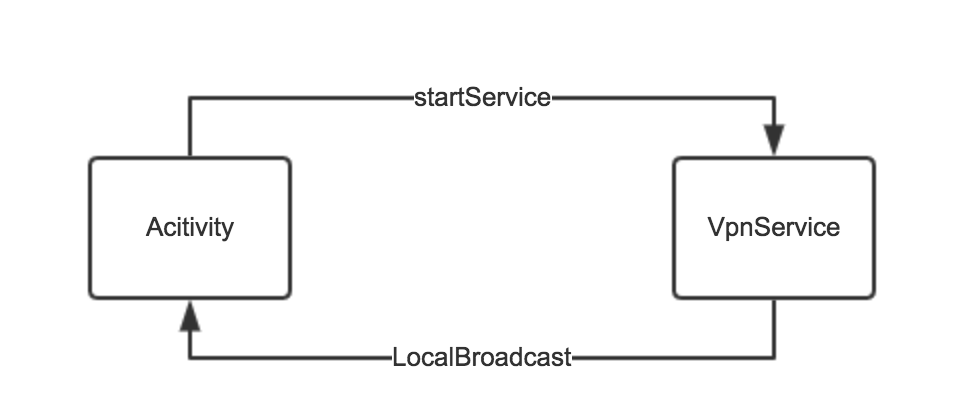
\includegraphics[width=.8\textwidth]{image_intent_commuciate.png}
\caption{VpnService与Activity通信图}\label{fig:1}
\end{figure}

Activity是界面,VpnService是后台服务。VpnService在工作时,Activity可能并不存在,如果需要传递信息给Activity,在其不存在时,就应该忽略这条信息;而Activity运行时,调用VpnService时,如果VpnService尚未运行,则需要创建VpnService。因此才采用了不同的通信机制:
Activity注册本地本地广播接收器,VpnService通过sendBroadcast(Intent)方法发送本地广播,如果Activity存在并且正在监听,则会收到信息;
Activity通过调用startService(Intent)发送Intent到VpnService,如果VpnService没有启动则会启动,已经启动则会通知现有的Service。

Intent中可以携带信息,通过实现预定好的协议,可以从Intent携带的信息中得知命令。我们约定协议如下:
\begin{itemize}
    \item run     启动VPN后台服务,并进行请求权限等准备工作,进入就绪状态
    \item start   建立VPN连接,开启防火墙
    \item reload  重新载入防火墙配置
    \item stop    断开VPN连接,暂停防火墙,回到就绪状态
    \item stats   诊断状态,使防火墙将自身状态和日志输出到控制台
\end{itemize}

\section{VpnService状态机}

实现VpnService代码量较多,为了使逻辑清晰,采用状态机的设计。包含以下状态:
\begin{itemize}
    \item none          未就绪状态,VpnService不可用
    \item waiting       等待状态,用户已经许可了权限,但并没建立VPN连接
    \item enforcing     启用状态,VPN连接已建立,VPN正在运行
    \item stats         报告状态,VpnService需要报告当前信息,用于诊断
\end{itemize}

这些状态在使用run, start, reload, stop, stats这些命令时会发生状态迁移,状态迁移图如\autoref{fig:3} 所示:

\begin{figure}[h!]
\centering
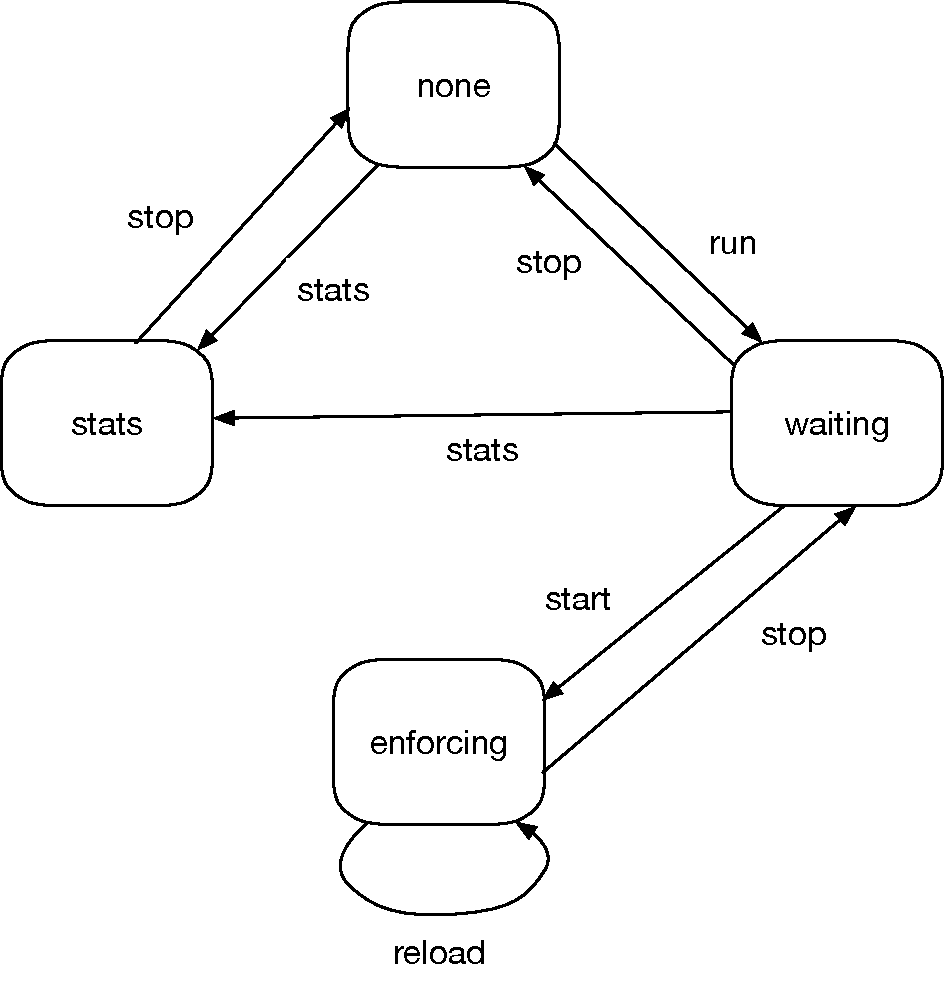
\includegraphics[width=.6\textwidth]{state_machine}
\caption{VpnService状态迁移图}\label{fig:3}
\end{figure}


\section{防火墙规则设计}

由于支持多种特殊情况下的组合防火墙规则,防火墙规则较为复杂,在实现上设计了一个Rule类用来储存运行时的规则信息:

\begin{lstlisting}[language=java]
    public class Rule {
        public PackageInfo info;
        public String name;
        public String description;
        public boolean system;
        public boolean internet;
        public boolean enabled;
        public Intent launch;
        public Intent settings;
        public Intent datasaver;
        public boolean pkg = true;

        public boolean wifi_default = false;
        public boolean other_default = false;
        public boolean screen_wifi_default = false;
        public boolean screen_other_default = false;
        public boolean roaming_default = false;

        public boolean wifi_blocked = false;
        public boolean other_blocked = false;
        public boolean screen_wifi = false;
        public boolean screen_other = false;
        public boolean roaming = false;

        public boolean apply = true;
        public boolean notify = true;

        public boolean relateduids = false;
        public String[] related = null;

        public float upspeed;
        public float downspeed;
        public float totalbytes;

        public boolean changed;

        public boolean expanded = false;
    }
\end{lstlisting}

\section{数据库设计}

\subsection{数据库表设计}
防火墙的规则需要使用数据库来进行储存和管理。防火墙通过访问规则表来控制网络流量,访问规则表包括以下字段:

\begin{itemize}
    \item uid           用于唯一识别应用的id
    \item version
    \item protocol      规则适用的协议
    \item daddr
    \item dport

    \item time
    \item allowed
    \item block

    \item sent
    \item received
    \item connections
\end{itemize}

"CREATE TABLE access (" +
                " ID INTEGER PRIMARY KEY AUTOINCREMENT" +
                ", uid INTEGER NOT NULL" +
                ", version INTEGER NOT NULL" +
                ", protocol INTEGER NOT NULL" +
                ", daddr TEXT NOT NULL" +
                ", dport INTEGER NOT NULL" +
                ", time INTEGER NOT NULL" +
                ", allowed INTEGER NULL" +
                ", block INTEGER NOT NULL" +
                ", sent INTEGER NULL" +
                ", received INTEGER NULL" +
                ", connections INTEGER NULL" +
                ");";

\subsection{数据库的实现}

   Android系统提供了SQLite数据库的支持,使用相关系统API即可实现数据库操作。对于操作数据库,需要实现如下一个类:

\begin{lstlisting}[language=java]
        public class DatabaseHelper extends SQLiteOpenHelper {

            @Override
            public void onCreate(SQLiteDatabase db) {
                Log.i(TAG, "Creating database " + DB_NAME + " version " + DB_VERSION);
                createTableLog(db);
                createTableAccess(db);
                createTableDns(db);
                createTableForward(db);
            }

            @Override
            public void onUpgrade(SQLiteDatabase db, int oldVersion, int newVersion) {

            }

        }
\end{lstlisting}

   该类用户每次打开数据库时,如果数据库表结构没有创建,会调用onCreate中相关代码进行创建表结构,如果数据库表版本不是最新,调用onUpgrade进行数据表版本的升级。
   打开数据库以后,可以进行数据库的读写操作。
   如下列代码可以实现从数据读取规则:

\begin{lstlisting}[language=java]
    lock.readLock().lock();
    try {
        SQLiteDatabase db = this.getReadableDatabase();
        return db.query("access", null, "block >= 0", null, null, null, "uid");
    } finally {
        lock.readLock().unlock();
    }
\end{lstlisting}

   下列代码更新了一条规则:

\begin{lstlisting}[language=java]
    lock.writeLock().lock();
    try {
        SQLiteDatabase db = this.getWritableDatabase();
        db.beginTransactionNonExclusive();
        try {
            ContentValues cv = new ContentValues();
            cv.put("allowed", packet.allowed ? 1 : 0);
            cv.put("uid", packet.uid);
            cv.put("version", packet.version);
            cv.put("protocol", packet.protocol);
            cv.put("daddr", dname == null ? packet.daddr : dname);
            cv.put("dport", packet.dport);

            rows = db.update("access", cv, "uid = ? AND version = ? AND protocol = ? AND daddr = ? AND dport = ?", new String[]{
                            Integer.toString(packet.uid),
                            Integer.toString(packet.version),
                            Integer.toString(packet.protocol),
                            dname == null ? packet.daddr : dname,
                            Integer.toString(packet.dport)});

            db.setTransactionSuccessful();
        } finally {
            db.endTransaction();
        }
    } finally {
        lock.writeLock().unlock();
    }
\end{lstlisting}


\section{应用配置设计}

应用需要储存用户的配置,我们为方便用户,提供了以下全局设置选项:
\begin{itemize}
	\item 默认阻止Wi-fi网络        boolean
	\item 默认阻止移动网络          boolean
	\item 亮屏时默认允许Wifi网络     boolean
	\item 亮屏时默认允许移动网络      boolean
	\item 默认阻止漫游              boolean
\end{itemize}
此外,应用还需要储存一些状态信息,这些信息不适合存入数据库,比如VPN是否启用,用户是否在应用市场为我们的应用评过分,我们需要采取一些轻量级非关系型的存储方案。

\subsection{SharePreference储存}

SharePreference是Android系统提供的一种简单的Key-Value持久化机制。广泛用于储存应用配置。它在实现上创建了一个XML文件用来储存Key-Value,储存位置根据SharePreference是否私有来定,如果是私有的,将会储存在应用程序自己的沙箱中,无法被其他应用访问。具体使用方式如下:

如下代码会打开默认的SharePreference储存空间,并从中读取信息:

\begin{lstlisting}[language=java]
    final SharedPreferences prefs = PreferenceManager.getDefaultSharedPreferences(this);
    boolean enabled = prefs.getBoolean("enabled", false);
    boolean default_wifi = prefs.getBoolean("whitelist_wifi", true);
    boolean default_other = prefs.getBoolean("whitelist_other", true);
\end{lstlisting}

以下代码可以储入信息:

\begin{lstlisting}[language=java]
    final Editor editor = prefs.edit();
    editor.putBoolean("enabled", true);
    editor.putString("user_name","Carlos");
    editor.commit();
\end{lstlisting}

\subsubsection{SharePreference存储设计}

应用主要包含多级的配置结构,以及一些单列的配置文件,对此我们设计其结果如下图所示:

\todo[inline]{增加SharePrefenrence图}

\todo[inline]{列举设置条目}

\chapter{系统测试}

\todo[inline]{列出兼容性测试项目表},说明要兼容的项和原因,解释新功能,截图证明兼容性
\todo[inline]{列出功能测试项目表},UI截图证明
\todo[inline]{列出性能测试项目表},列出数据




\chapter{结论}

\backmatter

\begin{ack}
致谢正文。
\end{ack}

\bibliography{ref-example}

\appendix

\chapter{这是一个附录}\label{appendix:1}
附录正文。


\end{document}
\endinput